\section{Synthesis of the equivalent transmission for full pupil illumination}
\label{sec:pupil_stitching}

The reflectivity of the telescope and the transmission of the filters
both exhibit a distinct radial dependency. Although the filter
transmission dependence is expected due to its interferometric nature,
the origin of the telescope reflectivity dependence remains
unclear. Despite this, we can construct an empirical model that
assumes smooth transitions between measurements and calculate the
theoretical "full pupil" transmission by averaging the model over the
illuminated portion of the primary mirror. These two steps are
necessary to achieve sub-percent color accuracy and sub-nanometer
precision in central wavelengths determination.

We also estimate statistical and systematic errors on the final
transmission curves, and propagate them through the analysis process. A
better understanding of these errors in interpreting broadband
photometry is obtained using the spectrophotometric standard star
G191B2B as a sample star.


\subsection{Radial model of the instrument transmission}
\label{sec:model}

The open transmission of the telescope is modeled as a smooth 2D
function of wavelength and incidence angle. The function is defined on
a basis of cubic B-splines, with \num{35} regularly spaced wavelength
nodes covering the range from \SIrange{350}{1100}{nm}, and two nodes
at angles corresponding to the inner and outer edges of the
occultation-free primary mirror, ranging from \SIrange{1.97}{7.24}
{\degree}. These angles represent radii of \SIrange{55}{203}{mm} for a
primary mirror with a focal length of \SI{1600}{mm}.

For data acquired using a filter, we multiply the open transmission
model by a model of the interference filter transmission, defined as
follows:
\begin{equation}
  \label{eq:filtertransmission}
T(\lambda, \theta) = \mathcal T\left(\frac{\lambda}{\sqrt{1 -
    (\sin(\theta) / n_\text{eff})^2}}\right)\,.
\end{equation}
Here, $n_\text{eff}$ is an effective index for the filter,
and $\mathcal{T}$ is a piece-wise linear function of wavelength. The piece-wise
linear function is initially created with \num{150} regularly spaced
nodes between \SIrange{350}{1100}{nm}, providing a general resolution
of \SI{5}{nm}. In cases where more precision is needed, we further
refine the grid by equally splitting intervals where the local mean
chi-square exceeds the global mean chi-square by more than three
standard deviations. This process is repeated four times to ensure
that filter fronts are typically modeled with up to approximately
\SI{0.3}{nm} resolution.


In the specific case of the  grating zeroth and first orders, the photometry is
adjusted using a cubic B-spline model with \num{105} nodes in
wavelength.

The composite model is fit to dataset No.~2, which includes data
from four different radii and successive observations without filters
or with all seven filters and the grating. The baseline model has
\num{1979} free parameters: \num{148} for the open transmission,
approximately $6\times165$ for each of the $ugrizy$ filters, and
\num{420} for each of the grating orders. Unfortunately, the blue edge
of the $u$-band filter cannot be accurately measured with this
data. Fit results are displayed in
Fig.~\ref{fig:lambdathetafitresults}.

\begin{figure*}
  \centering
  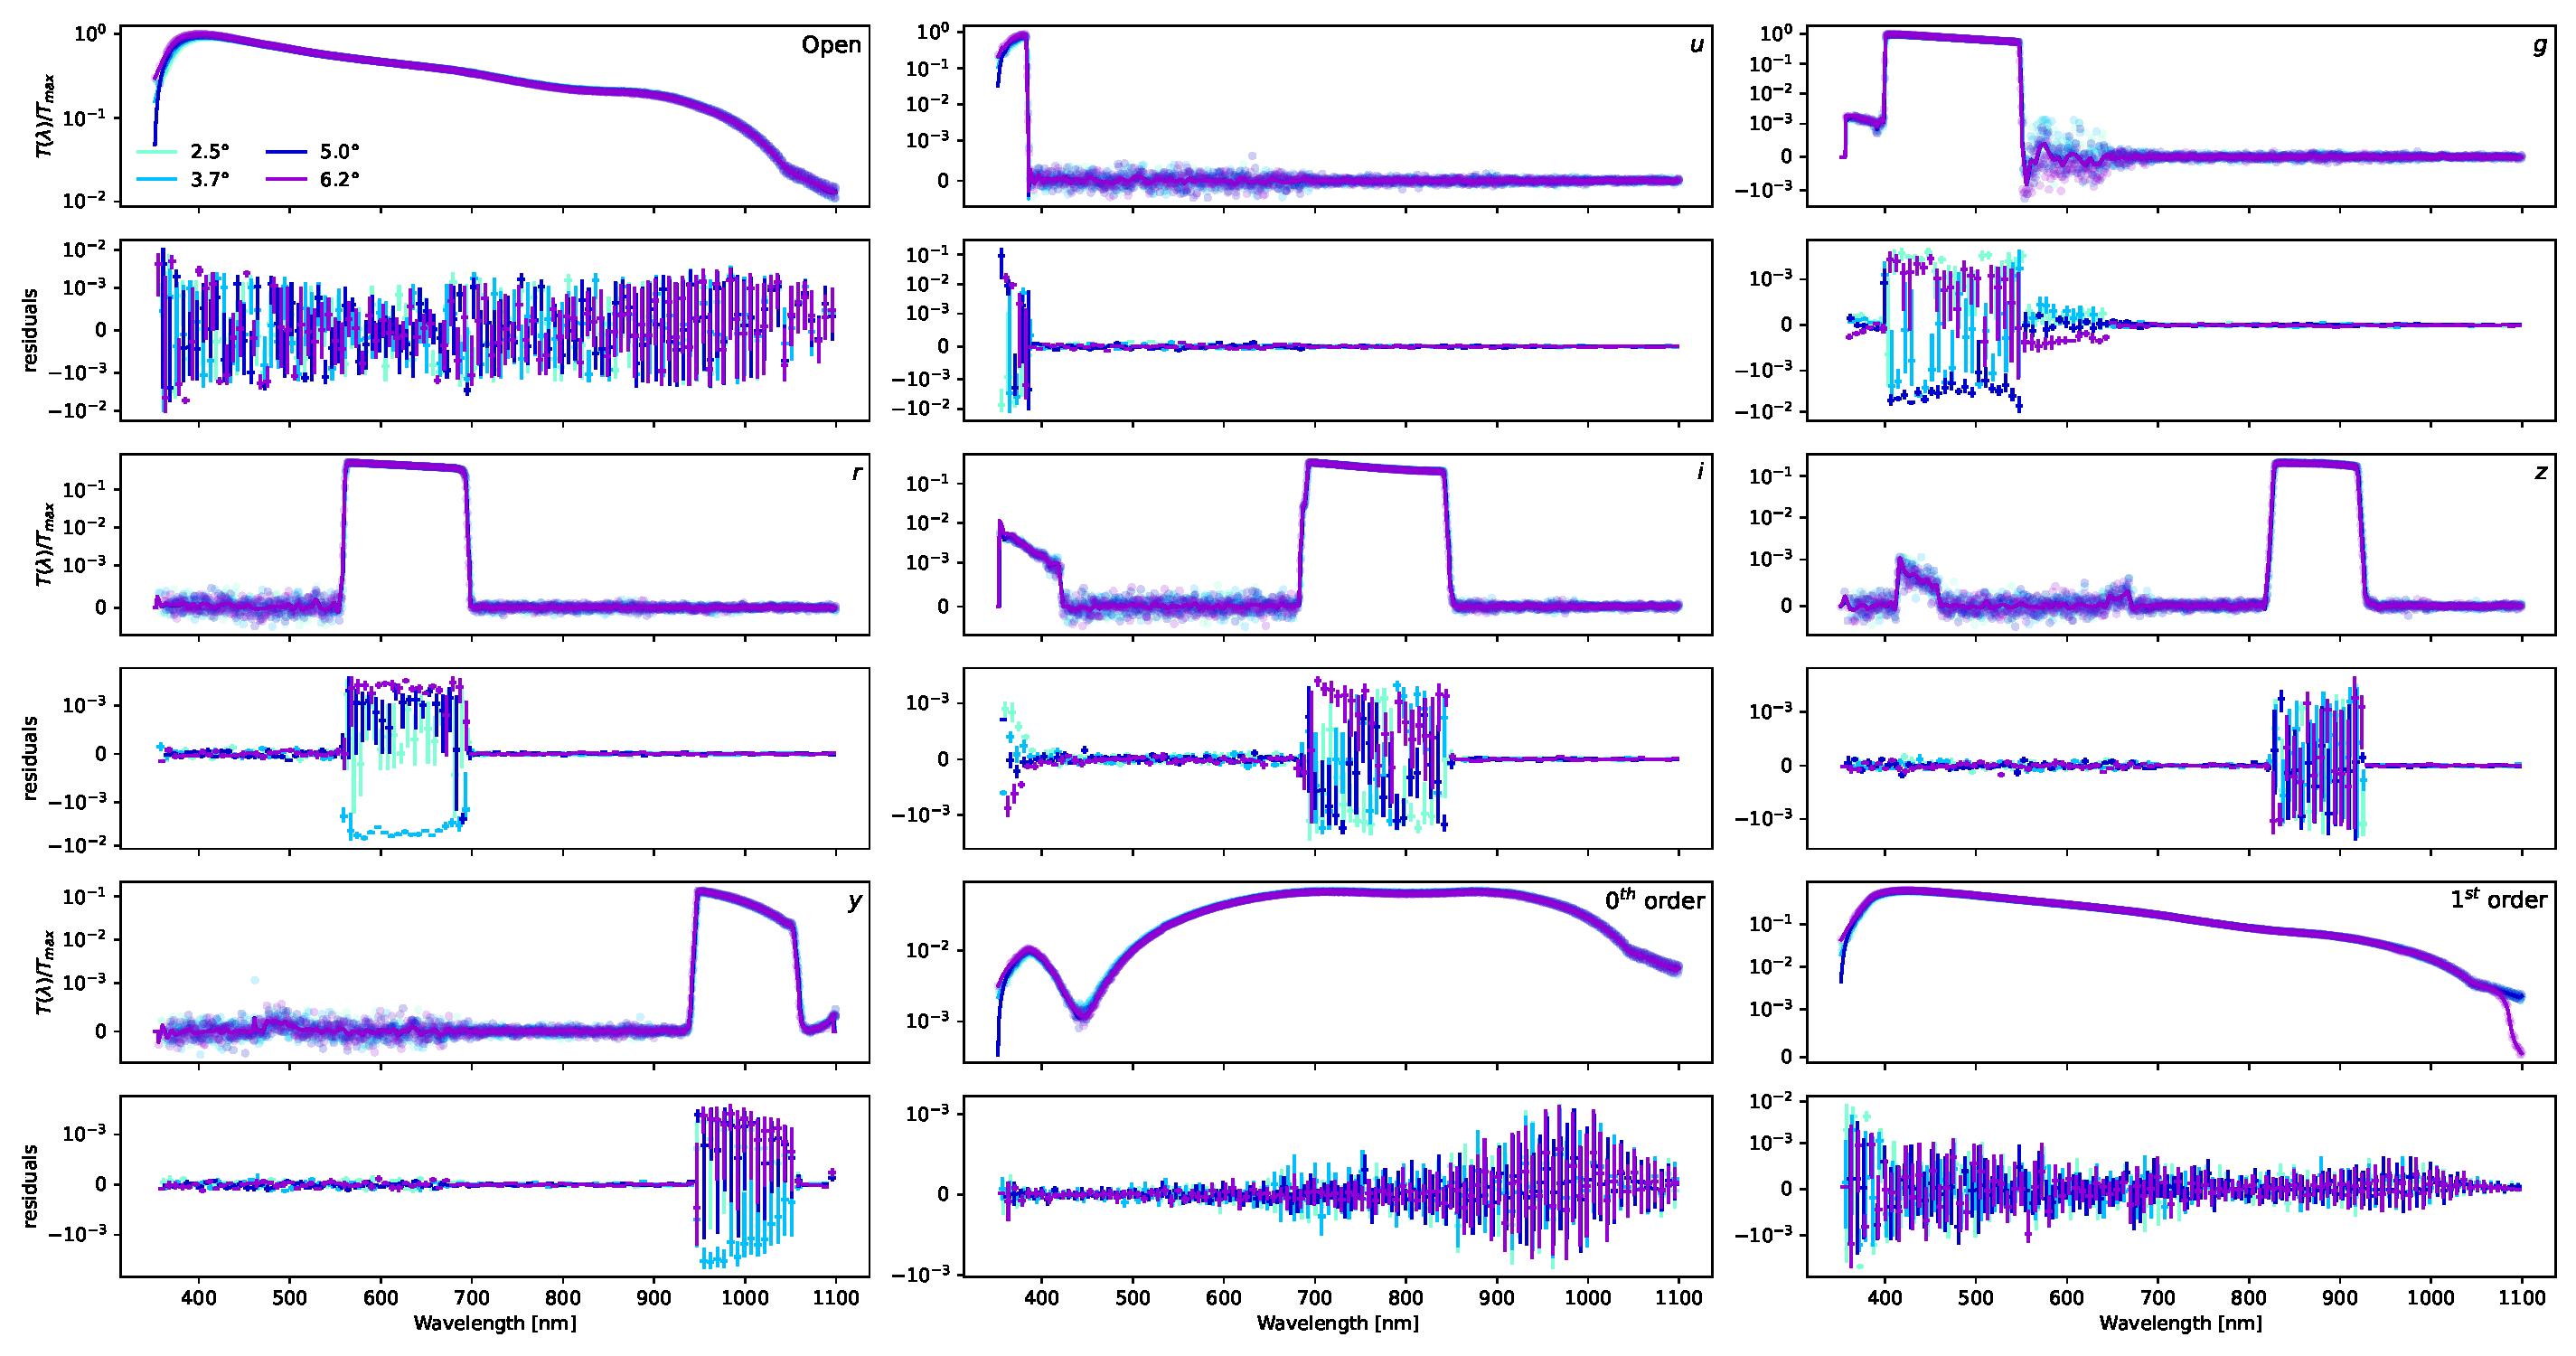
\includegraphics[width=1\linewidth]{./fig/lambdathetafitresults.pdf}
  \caption{Model of the wavelength and radial dependency of the
    StarDICE response to CBP illumination $R(\lambda)$. Each panel
    display the raw measurements at the 4 sampled positions for each of
    the filter configurations: no filters (Open), with one of the 6
    photometric filters ($ugrizy$) or with the grating looking either
    at the zeroth order or the first order spots. The panel
    immediately below each panel display the residuals to the
    model as a fraction of the data. For easy comparison, all panels are normalized to the peak
    of the response, which occurs in the open configuration at
    $\lambda = \SI{398}{nm}$ and $\theta = \SI{6.2}{\degree}$.
    %\textbf{SZF: les résidus de l'open transmission sont sur une échelle différente des autres}
 }
  \label{fig:lambdathetafitresults}
\end{figure*}


\begin{figure}
  \centering
  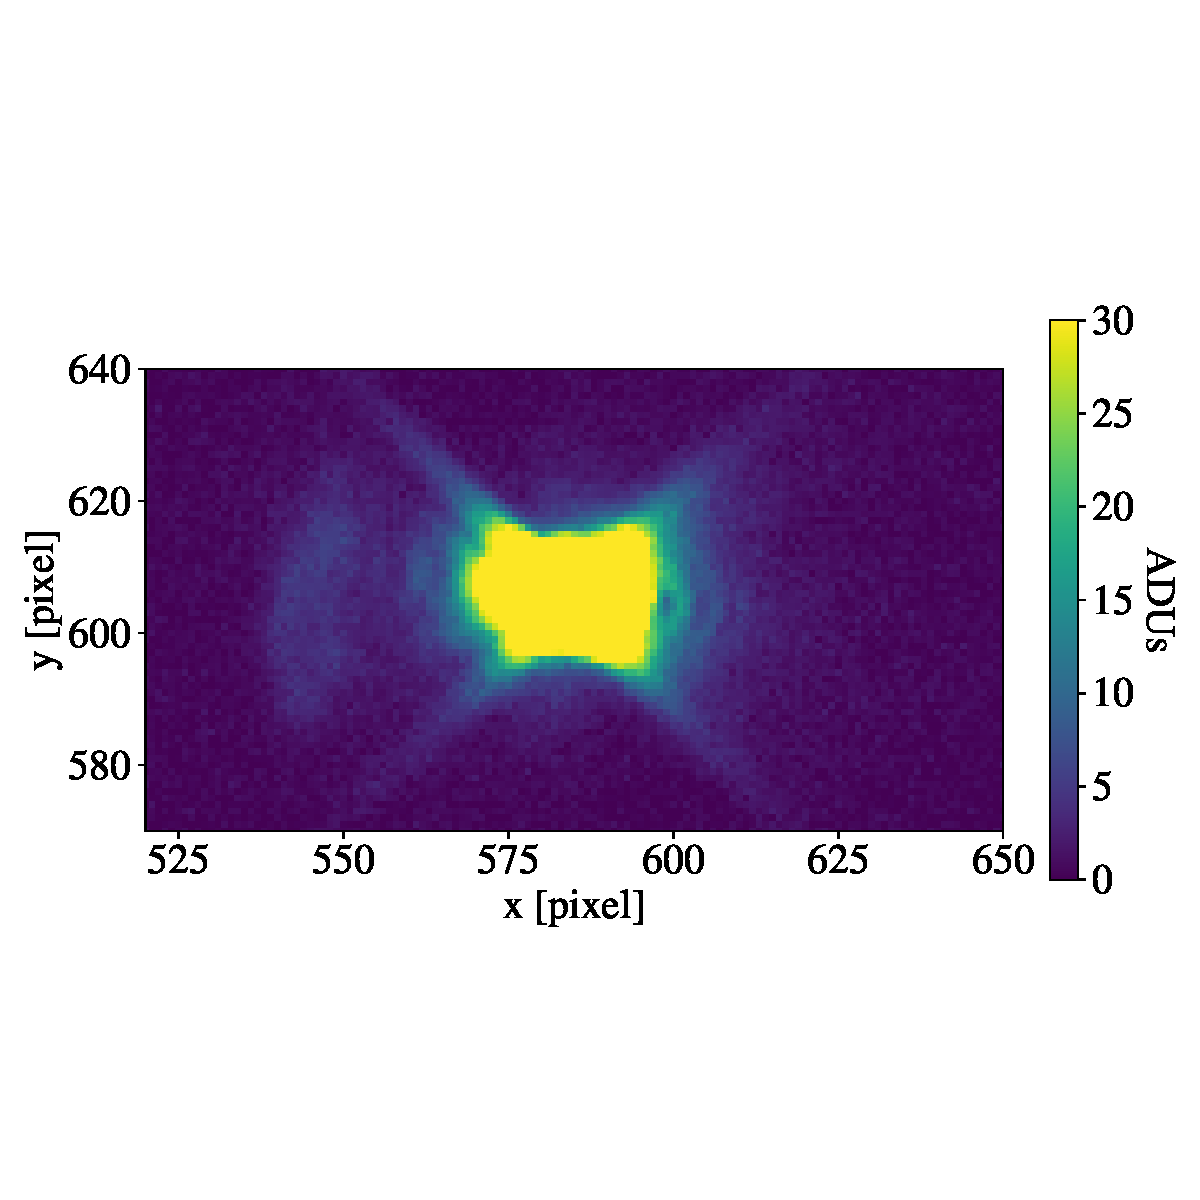
\includegraphics[width=1\linewidth]{fig/diffraction_dust.pdf}
  \caption{Diffraction rings due to the presence of a dust spot on the
    r filter, intercepting the CBP beam.}
  \label{fig:dust}
\end{figure}


Overall, the model provides a satisfactory description of the
dataset. The most significant discrepancy is a noticeable gray
decrease in the transmission of the $r$ filter for the sample
measurement at \SI{3.7}{\degree} with respect to the average of the
other three.  After investigating this issue, we identified that the
corresponding images displayed a diffraction figure consistent with
the presence of a dust particle on the filter surface intercepting the
CBP beam, visible in Figure~\ref{fig:dust}. Based on the approximate area of the beam spot
($\sim$\SI{12}{\milli\metre\squared}), and the estimated particle size range (between
\SIrange{200}{300}{\micro\metre}), we calculated a potential decrease
in transmission for this specific partial illumination of the primary
mirror of up to \SI{0.6}{\percent}. This value is in good agreement
with the observed decrease. Similar discrepancies were found for some
observations in $u$, $g$, and $y$ bands, although determining particle
sizes from diffraction features was not possible in these cases. We
attribute these discrepancies to dust contamination on the filter
surface as well.

The top panel of Fig.~\ref{fig:metrics} shows the difference between
the transmission integral for measurements and the model at each
position, helping readers better visualize the 'gray'
discrepancies. The standard deviation of the model/measurement
discrepancies is \SI{10.2}{mmag}. Considering this value as an
estimate of dust-induced dispersion, we can deduce that the
corresponding uncertainty for per-filter normalization of the model
(averaging 4 independent samples) is approximately $\SI{5}{mmag}$.

This noise could be decreased by averaging more sample measurements of
the mirror. In our case 4 additional positions were sampled as part
of run 3 (see table~\ref{tab:schedule}). However, while measurements of run No.~2 were carefully taken to sample the mirror from the outer
edge to the inner edge along a radius with separations provided by the
mount encoders, the other measurements were positioned semi-randomly
with the idea that the position of the CCD-window ghost in the images
will enable precise determination of the position of the beam in the
mirror. Two issues were overlooked at this stage which complicated the
determination of the geometry from the position of the ghosts: (1) The
wedge of the CCD window and (2) the ghost position dependence on the
conjugation relation between the CBP and the telescope which is only
approximately known. The complexity of including those parameters in a
full model of the telescope+CBP sets the analysis of those data out of
the scope of the current paper.

The bottom panel in Fig.~\ref{fig:metrics} displays the difference
between the measured central wavelength and the model-predicted value
for all 4 radius positions. The model accurately reproduces the
central wavelengths of all filters with a standard deviation of only
$\SI{0.13}{nm}$. This represents an improvement by an order of
magnitude compared to a model that neglects wavelength shift
considerations due to the light incidence angle on the filter, highlighting the importance of including this effect
in the StarDICE response model.

\begin{figure}
  \centering
  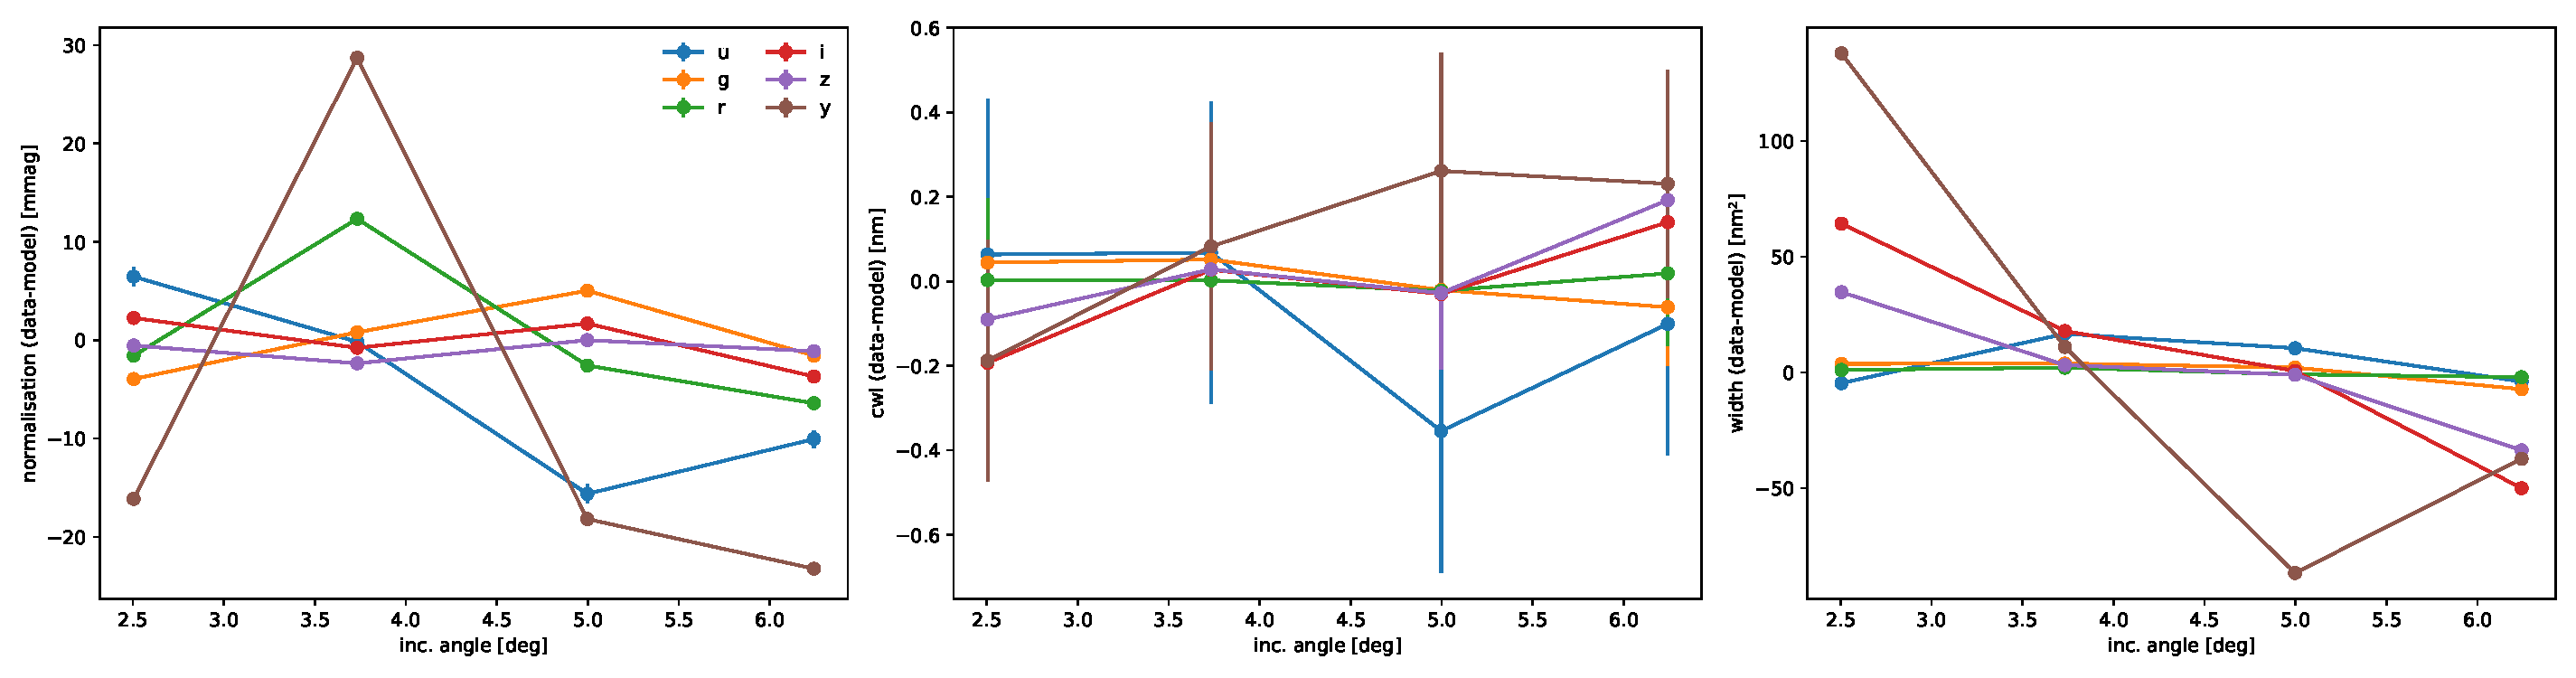
\includegraphics[width=1\linewidth]{fig/metrics.pdf}
  \caption{Discrepancies between model and raw measurements at
    different mirror locations summarized according to 2 metrics:
    \emph{Top:} relative difference in the integral of the passband,
    expressed in millimagnitudes; \emph{Bottom:} relative difference
    in central wavelength computed as the barycenter of the passband.}
  \label{fig:metrics}
\end{figure}

\subsection{Full pupil synthetic transmission curves}

The full pupil transmission is synthesized by numerically averaging
the above model assuming that the pupil is a perfect annulus with an
inner radius of \SI{55}{mm} and an outer radius of \SI{203}{mm},
corresponding to an effective mirror area of \SI{1202}{cm^2}. The
rectangle rule with 100 evenly sampled points in radius has been used
for the averaging. The curves have been normalized using the CBP
response from Sect.\ref{sec:cbp}. The resulting transmission curves
are shown in Fig.~\ref{fig:fullpupiltrans}.
\begin{figure}
  \centering
  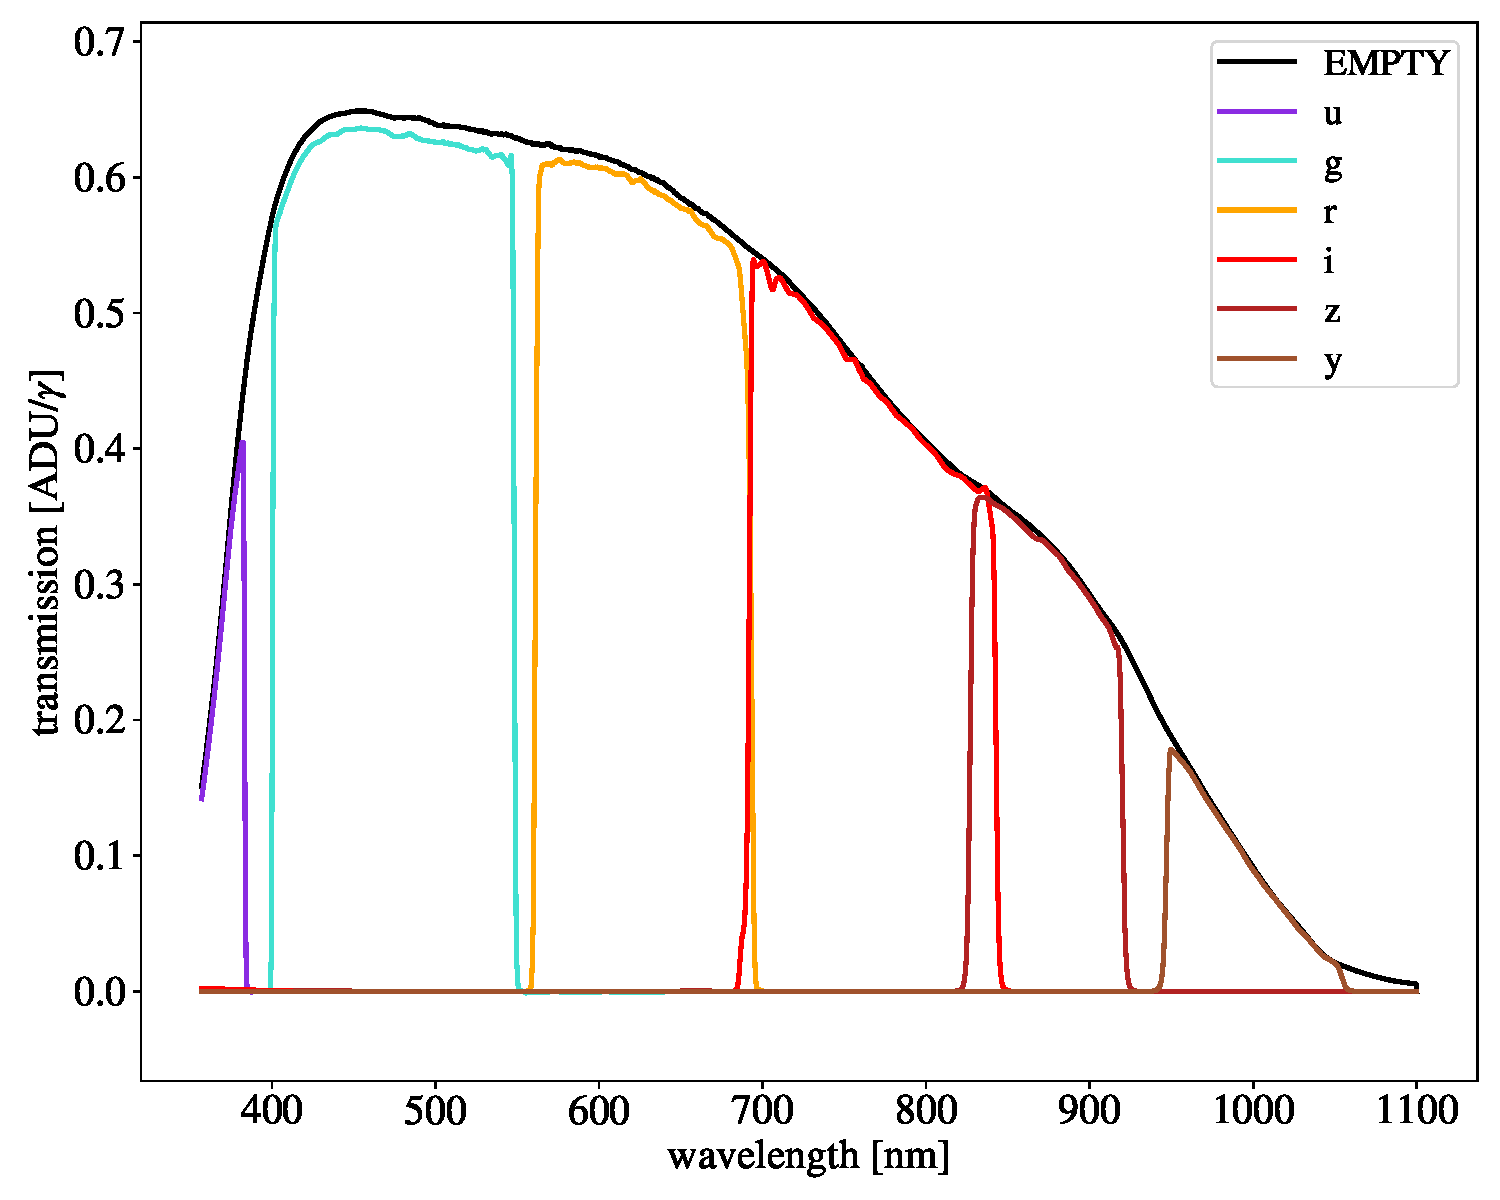
\includegraphics[width=1\linewidth]{fig/fullpupill.pdf}
  \caption{Full-pupil transmission curves for the StarDICE instruments.}
  \label{fig:fullpupiltrans}
\end{figure}


\subsection{Final uncertainty budget}
\label{sec:final_uncertainty_budget}

The impact of the uncertainties in our determination of the full-pupil
transmission curves depend on the application. We first consider the
use of the CBP as the sole source for absolute calibration of the
instrument response and then its use in conjunction with a broadband
star-like calibration light source.

\subsubsection{Uncertainties in absolute fluxes}
\label{sec:absolute}

The first obvious application is to take
each curve as an absolute calibration of the instrument throughput and
use it to interpret broadband fluxes measured by this instrument,
according to the equation:
\begin{equation}
  \label{eq:mb}
  \phi_b = \int_\lambda  R_b(\lambda) A(\lambda) S(\lambda) \lambda d\lambda
\end{equation}
where $R_b$ is the full pupil response curve of the instrument
synthesized previously, $S$ is the top of the atmosphere spectrum of
the target and $A$ is the atmospheric transmission for this
observation. Setting aside the question of the atmospheric
transmission, the error $\delta R_b$ on the passband will translate
into an error on the synthesized flux $\delta \phi$, whose magnitude
depends on the spectrum of the object. As an illustration we
propagated all our uncertainties to the synthetic fluxes of the
primary spectrophotometric standards G191B2B. We report the results in
Table~\ref{tab:budget} as the relative uncertainty on the broadband
flux $\sigma(\delta \phi)/\phi$ for each band, with one line per
contributions. The table does not include the uncertainty on the gray
scale, mainly coming from the uncertainty in the effective area of the
telescope which cannot be determined accurately with such a setup. 

% Pas de gray scale
\begin{table}
  \centering
  \caption{Relative uncertainty in the synthetic broadband fluxes of
    G191B2B, split by contributions, in permil.}
  \label{tab:budget}
  \begin{tabular}{@{}l@{}rrrrrr@{}}
    \toprule
    \toprule
    Source & $u^\dag$ & $g$ & $r$ & $i$ & $z$ & $y$ \\
    & $[\text{\textperthousand}]$ & $[\text{\textperthousand}]$ & $[\text{\textperthousand}]$ & $[\text{\textperthousand}]$ & $[\text{\textperthousand}]$ & $[\text{\textperthousand}]$\\
    \midrule
    StarDICE & 0.5 & 0.2 & 0.2 & 0.3 & 1.0 & 3.8 \\
    $\Esolar$ & 1.6 & 0.1 & 0.1 & 0.1 & 0.1 & 0.1 \\
    CBP & 2.2 & 0.5 & 1.2 & 0.0 & 0.0 & 0.1 \\
    \midrule
    Stat (total) & 2.7 & 0.5 & 1.2 & 0.3 & 1.0 & 3.8 \\
    \midrule
    Scattered light & 2.7 & 3.1 & 3.8 & 4.3 & 4.8 & 5.3 \\
    Repeatability & 0.8 & 0.4 & 0.5 & 1.1 & 1.1 & 1.1 \\
    Linearity & 0.2 & 0.2 & 0.3 & 0.5 & 0.5 & 0.5 \\
    Contamination & 4.4 & 0.6 & 0.8 & 0.1 & 0.1 & 0.1 \\
    Mirror sampling noise & 5.4 & 5.4 & 5.4 & 5.4 & 5.4 & 5.4 \\
    NIST photodiode & 0.2 & 0.1 & 0.0 & 0.0 & 0.0 & 0.1 \\
    Solar cell temperature & 0.0 & 0.0 & 0.0 & 0.0 & 0.0 & 3.9 \\
    Wavelength calibration & 0.7 & 0.6 & 0.5 & 0.4 & 0.3 & 0.3 \\
    \midrule
    Syst (total) & 7.6 & 6.3 & 6.7 & 7.1 & 7.4 & 8.7 \\
    \midrule
    Total & 8.0 & 6.3 & 6.8 & 7.1 & 7.5 & 9.4 \\
    \bottomrule
  \end{tabular}
  \tablefoot{$^\dag$Our measurement does not capture the blue side of the $u$ band filter. We propagate uncertainties as if the transmission was dropping to 0 at the edge of the measurement to illustrate the performances that would be obtained from a complete measurement. For all practical purposes, however, the actual $u$ band transmission cannot be determined from the existing measures.}
\end{table}

The dominant contributor to the uncertainty in our flux reconstruction
is the mirror sampling noise. With the CBP beam sampling only a small
fraction of the primary mirror, and therefore a small fraction of the
filters, any inhomogeneity in the transmission of the filter ends up
causing a noise in the band-to-band ratio of transmissions. This noise
decreases with more sampling points on the primary mirrors, at a large
observational cost.

The next significant issue is the difficulty of getting rid of
non-collimated (scattered) light during the calibration of the CBP on
the solar-cell array. A natural way to deal with this issue would be
to significantly increase the solar-cell CBP distance. In our case, however, the beam created by the \bpinhole pinhole already barely fit
inside the footprint of the solar cell. Increasing the solar-cell CBP
distance would have caused issues for the collimated beam calibration in exchange
for getting rid of the non-collimated light.

Some caution needs to be paid to changes in the working temperature
of photodiodes when calibrating the $y$ band. In our current measurement,
the uncertainty in the difference in temperature between the
calibration of the solar cell and its use to calibrate the CBP is
quite large (\SI{1.6}{\celsius}). This has easily been fixed in the latter
iteration of the solar-cell design by including temperature sensors
directly cell enclosure.

Our mitigation procedure for the contamination of the beam by light
at different wavelengths is found satisfactory for all bands but $u$. This
is due to the remaining uncertainties in the determination of the
phosphorescence contribution in the integrating sphere.

\begin{figure}
  \centering
  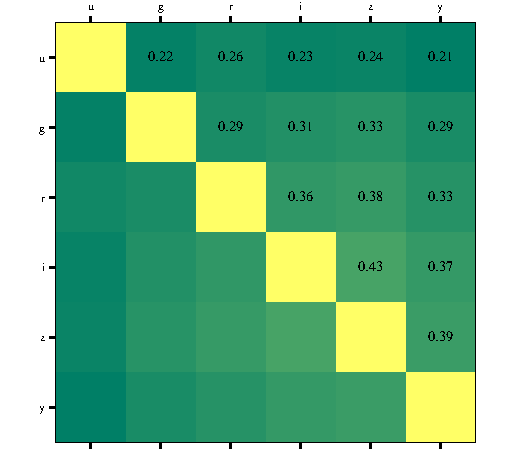
\includegraphics[width=1\linewidth]{fig/bandcorrelation.pdf}
  \caption{Correlation of the uncertainties on the synthetic fluxes of G191B2B.}
  \label{fig:correlation}
\end{figure}

Lastly, most systematic uncertainties have modes coherent across
wavelengths. As a result, the errors induced on broadband magnitudes
are correlated across bands, with typical correlation levels in the
20-40\% range. The correlation matrix resulting from the full
propagation of uncertainties identified in Table~\ref{tab:budget} is
displayed in Fig.~\ref{fig:correlation}. Again, we do not account for
the uncertainty in the gray scale which is perfectly correlated
between all bands and would dominate the uncertainty budget.

\subsubsection{Uncertainties in relative fluxes}
\label{sec:relative}

The more common application of telescope transmission measurements is
to rely on the transmission curves to predict actual
observations of a spectrophotometric standard of known flux and
determine an independent re-calibration factor for each band. The
errors on the interpretation of observations of another object will
then depend on the difference in color between the object and the
spectrophotometric standard, canceling for objects whose spectrum is
very similar to the spectrum of the standard.

For the StarDICE telescope, the role of photometric standard is played
by a collection of narrow-spectrum LEDs, whose observations set the
absolute normalization of each band. The telescope is then used to
observe CALSPEC standard stars and precisely measure their broadband
fluxes, anchoring them to the LEDs absolute calibration.
In this operation, all uncertainties which mostly impact the
normalization of the passbands cancels out. In order to illustrate the
impact of the uncertainties in our passband determination in this
case, we modeled the spectrum of 6 calibration LEDs as Gaussian shapes
centered on the central wavelength of each filter with a full-width
half-maximum of 7\% in wavelength. 
To simulate the effect of the passband recalibration on LED
observations, we propagate the uncertainties on the \emph{ratios} of
broadband fluxes between the LEDs and G191B2B. The results are
presented in Table \ref{tab:led}. As expected, most broadband error
sources cancel out, resulting in an accuracy of the order of 1 permil,
matching the requirements for the StarDICE experiment.

In contrast, the sensitivity to wavelength calibration generally
increases in a way that depends on the spectra of the LEDs. The flux of
LEDs whose spectrum overlaps with the edges of the filters are more
strongly affected by wavelength calibration errors than LEDs whose
spectrum is largely contained in the filter passband. The design of
the StarDICE artificial star includes both cases, with the idea that
overlapping LEDs can provide a handle to test (or correct) for filter
front errors. Here we report sensitivity for non-overlapping LEDs
assuming no specific correction.

\begin{table}
  \centering
  \caption{Uncertainties in the flux of G191B2B after recalibration by observation of narrow-spectrum LEDs centered on the filter passband.}
  \label{tab:led}
  \begin{tabular}{@{}l@{}r@{}r@{}r@{}r@{}r@{}r@{}}
    \toprule
    Source & u & g & r & i & z & y \\
           & $[\text{\textperthousand}]$ & $[\text{\textperthousand}]$ & $[\text{\textperthousand}]$ & $[\text{\textperthousand}]$ & $[\text{\textperthousand}]$ & $[\text{\textperthousand}]$\\
    \midrule
    StarDICE & 0.2 & 0.3 & 0.2 & 0.2 & 0.5 & 1.8 \\
    $\Esolar$ & 0.4 & 0.1 & 0.1 & 0.1 & $<0.1$ & 0.1 \\
    CBP & 0.5 & 0.5 & 1.1 & $<0.1$ & $<0.1$ & $<0.1$ \\
    \midrule
    Stat (total) & 0.7 & 0.6 & 1.1 & 0.2 & 0.5 & 1.8 \\
    \midrule
    Scattered light & $<0.1$ & 0.1 & $<0.1$ & $<0.1$ & $<0.1$ & $<0.1$ \\
    Repeatability & $<0.1$ & $<0.1$ & 0.1 & $<0.1$ & $<0.1$ & $<0.1$ \\
    Linearity & $<0.1$ & $<0.1$ & $<0.1$ & $<0.1$ & $<0.1$ & $<0.1$ \\
    Contamination & 0.1 & 0.1 & $<0.1$ & $<0.1$ & $<0.1$ & $<0.1$ \\
    Mirror sampling noise & $<0.1$ & $<0.1$ & $<0.1$ & $<0.1$ & $<0.1$ & $<0.1$ \\
    NIST photodiode & 0.1 & 0.1 & $<0.1$ & $<0.1$ & $<0.1$ & 0.1 \\
    Solar cell temperature & $<0.1$ & $<0.1$ & $<0.1$ & $<0.1$ & $<0.1$ & 0.6 \\
    Wavelength calibration$^\dag$ & 0.3 & 0.5 & 0.6 & 1.1 & 0.9 & 1.4 \\
    \midrule
    Syst (total) & 0.3 & 0.5 & 0.6 & 1.1 & 0.9 & 1.5 \\
    \midrule
    Total & 0.8 & 0.8 & 1.3 & 1.1 & 1.1 & 2.4 \\
    \bottomrule
  \end{tabular}
  \tablefoot{$^\dag$The impact of wavelength calibration on
    led-calibrated fluxes depend significantly on the exact spectrum
    of the LEDs. The numbers presented come from a simulation of a
    realistic case, but the numbers for actual LEDs may differ.}
  
\end{table}


